\documentclass[a4paper, 12pt]{article}
\usepackage[utf8]{inputenc}
\usepackage[brazil]{babel}
\usepackage{amstext} 	% need for \text command
\usepackage{amsmath}    % need for subequations
\usepackage{amssymb}
\usepackage{graphicx}   % need for figures
\usepackage{verbatim}   % useful for program listings
\usepackage{color}      % use if color is used in text
\usepackage{subfigure}  % use for side-by-side figures
\usepackage{hyperref}   % use for hypertext links, including those to external documents and URLs
\usepackage{pictexwd}	% use for pictex graphs
\usepackage{booktabs}	% use for Publication quality tables in LaTeX

\author{\\ \\ \\ \\ \\ \\ Vítor M. Martins n USP 5463225\\
Matheus Filipe Andriolo Ramos n USP 6846112 \\ 
Danilo Siqueira Cesar n USP 6848705 \\  
Paulo Vinicius Miyuki Yamabe n USP 5432641 \\ \\ \\ \\ \\}
\title{Trabalho Peça GM}



\begin{document}

\begin{minipage}[b]{.1\linewidth} % A minipage that covers half the page
\centering

\includegraphics[width=2cm]{./fig/Logo_usp_jpg.pdf}
\end{minipage}
\hspace{1.1cm}
\begin{minipage}[b]{.5\textwidth}
\begin{center}
\normalsize{\textsc{Universidade de São Paulo}}\\
\small{\textsc{Escola Politécnica}}\\
\footnotesize{\textsc{Departamento de Engenharia Mecatronica}}\\[0.5cm]
\end{center}
\end{minipage}
\hspace{0.9cm} % To get a little bit of space between the figures
\begin{minipage}[b]{0.1\linewidth}
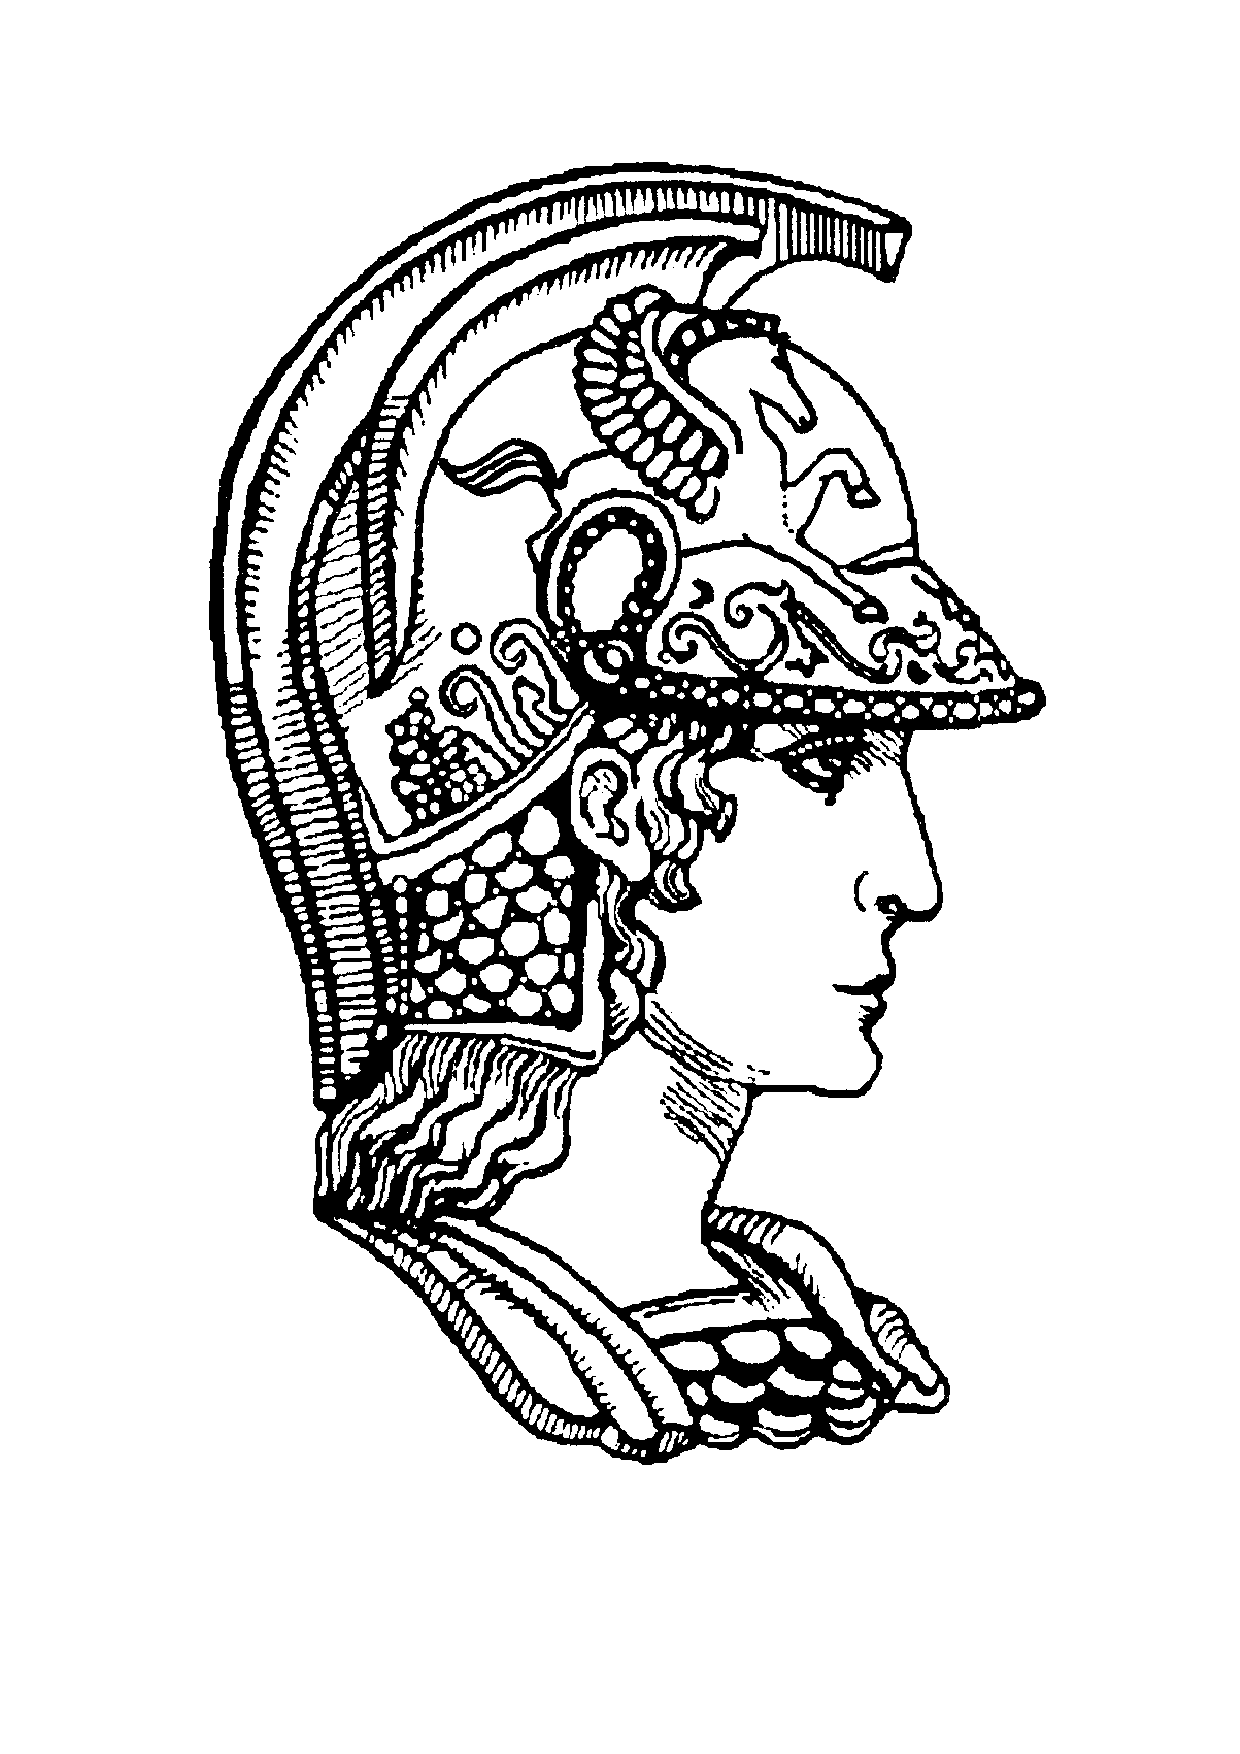
\includegraphics[width=2cm]{./fig/minerva.pdf}
\end{minipage}

\begin{center}

\textsc{\large PMR-2350 Exercicio para entrega }\\[2cm]


% Title
%\HRule \\[0.4cm]
%{ \Huge \bfseries Implementação da Pilha de Protocolos TCP/IP em FPGAs}\\[6.4cm]
% mudar o titulo
%\HRule \\[3.5cm]

{ \Huge \bfseries Peça Estampada}\\[3.4cm]

\begin{minipage}{0.5\textwidth}
\begin{flushleft}
\large \textbf{\emph{Alunos:}}\\
Vítor Matosinho Martins\\[0.1cm]
\large \textbf{\emph{Nº USP:}}
5463225\\


\end{flushleft}
\end{minipage}
\begin{minipage}{0.3\textwidth}
\begin{flushright}
\large \textbf{\emph{Professor:}} \\
Stipkovic\\
Prof Dr. Escola Politécnica
\end{flushright}
\end{minipage}\\[2.5cm]

\begin{center}
\large São Paulo, \today
\end{center}

\end{center}

\pagebreak

\tableofcontents
\listoffigures

\pagebreak

\section{Peça Estampada}

\begin{figure}[h]
\begin{center}
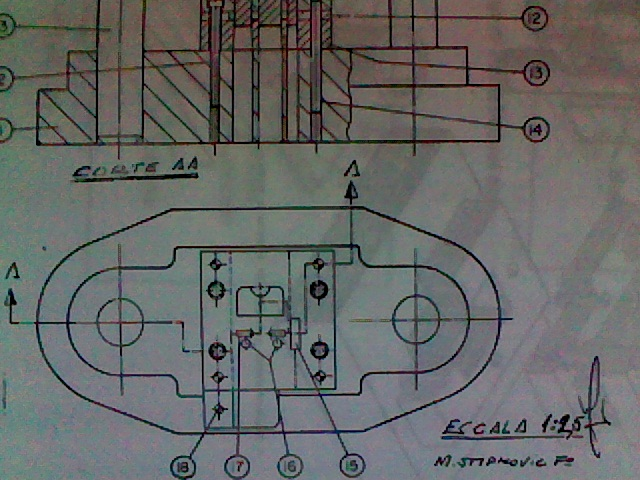
\includegraphics[scale=0.45]{./fig/111108-220046.jpg}
\caption{\label{fig:2}Máquina de estampagem.} 
\end{center}
\end{figure}

\begin{figure}[h]
\begin{center}
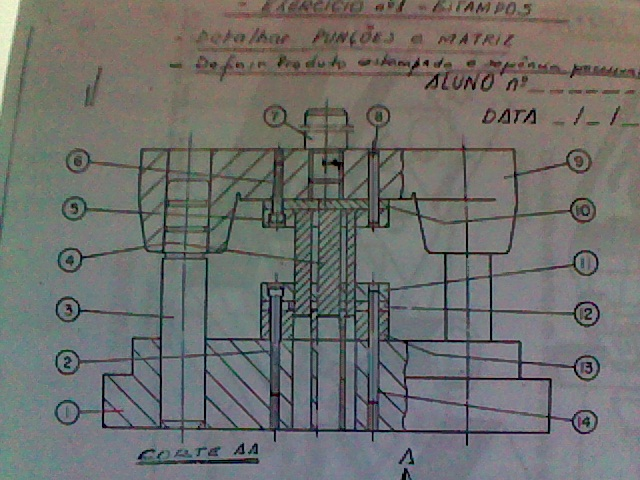
\includegraphics[scale=0.50]{./fig/111108-220105.jpg}
\caption{\label{fig:2}Máquina de estampagem.} 
\end{center}
\end{figure}



\begin{figure}[h]
\begin{center}
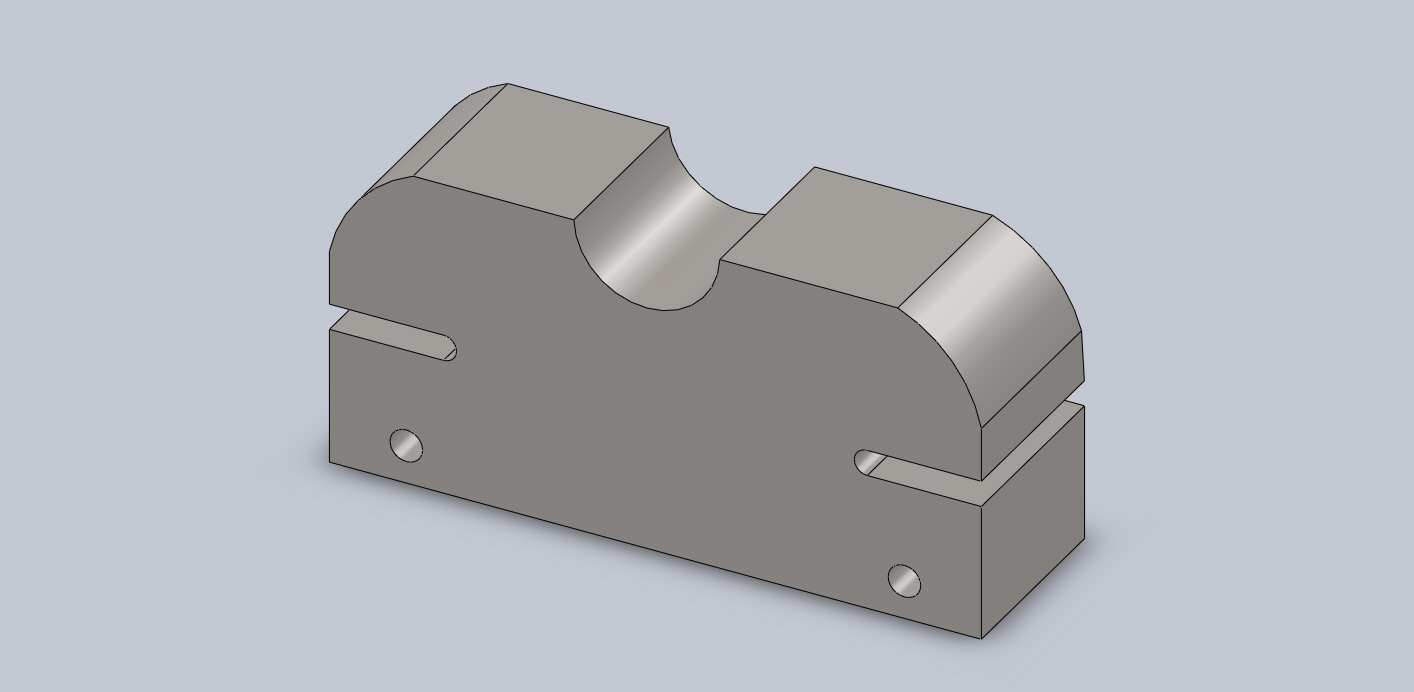
\includegraphics[scale=0.45]{./fig/peca_estampada-acoliga.jpg}
\caption{\label{fig:2}Peça que sai da máquina de estampagem.} 
\end{center}
\end{figure}

\begin{figure}[h]
\begin{center}
\includegraphics[scale=0.54]{./fig/peca_estampada_1.pdf}
\caption{\label{fig:2}Vista Trimétrica da Peça.} 
\end{center}
\end{figure}


\begin{figure}[h]
\begin{center}
\includegraphics[scale=0.78,angle=90]{./fig/peca_estampada.pdf}
\caption{\label{fig:2}Vistas Frontal, Superior e Lateral Direita.} 
\end{center}
\end{figure}





\pagebreak


\end{document}